\section*{Гармонический бустинг (Harmonic Boosting)}

Гармонический бустинг (Harmonic Boosting) представляет собой ансамблевый метод, целью которого является минимизация вклада моделей с высокой ошибкой путём взвешивания их предсказаний на основе гармонического среднего. Этот подход улучшает устойчивость ансамбля и снижает риск ухудшения качества из-за наличия "шумных" моделей.

\subsection*{Основная идея}

Гармоническое среднее даёт больший вес точным моделям и минимизирует влияние слабых или ошибочных предсказаний. Для \( n \) моделей ансамбля итоговое предсказание классификации вычисляется как:
\[
\hat{y} = \arg\max_{k} \left( \frac{n}{\sum_{i=1}^n \frac{1}{P_k(y_i)}} \right),
\]
где \( P_k(y_i) \) — вероятность принадлежности к классу \( k \), предсказанная \( i \)-й моделью.

Для регрессии итоговое предсказание:
\[
\hat{y} = \frac{n}{\sum_{i=1}^n \frac{1}{y_i}},
\]
где \( y_i \) — результат \( i \)-й модели.

\subsection*{Математическое обоснование}

Рассмотрим задачу регрессии. Пусть \( y_i \) — предсказание \( i \)-й модели, а \( e_i \) — её ошибка. Общая ошибка ансамбля определяется как:
\[
E = \frac{n}{\sum_{i=1}^n \frac{1}{e_i}}.
\]
Гармоническое среднее минимизирует \( E \), поскольку больший вес получают модели с меньшей ошибкой. Это свойство обеспечивает устойчивость ансамбля и снижает влияние "шумных" моделей.

Для классификации гармоническое среднее вероятностей используется в логарифмическом масштабе:
\[
\log P(C_k) = -\sum_{i=1}^n \frac{1}{\log P_k(y_i)}.
\]
Такой подход позволяет смягчить влияние моделей с крайне низкой вероятностью.

\subsection*{Алгоритм гармонического бустинга}

\textbf{Вход:}
\begin{itemize}
    \item Набор данных \( \mathcal{D} = \{(x_i, y_i)\}_{i=1}^m \),
    \item Количество слабых моделей \( T \),
    \item Функция потерь \( L(y, \hat{y}) \).
\end{itemize}

\textbf{Шаги алгоритма:}
\begin{enumerate}
    \item Инициализация ансамбля с первой моделью \( h_1 \), обученной на \( \mathcal{D} \).
    \item Вычисление весов для объектов в \( \mathcal{D} \) на основе обратной ошибки:
    \[
    w_j^{(t)} = \frac{1}{e_j^{(t)}},
    \]
    где \( e_j^{(t)} = L(y_j, h_t(x_j)) \).
    \item Построение новой модели \( h_{t+1} \) с учётом весов \( w_j^{(t)} \).
    \item Итоговое предсказание ансамбля:
    \[
    \hat{y} = \frac{n}{\sum_{i=1}^T \frac{1}{h_i(x)}}.
    \]
\end{enumerate}

\subsection*{Сравнение с другими методами бустинга}

В отличие от AdaBoost и градиентного бустинга, где обновление весов основывается на увеличении влияния сложных для классификации объектов, гармонический бустинг нацелен на минимизацию влияния моделей с высокой ошибкой. Это делает метод более устойчивым к выбросам и шуму.

\subsection*{Пример применения}

Рассмотрим задачу классификации на двух классах \( C_1 \) и \( C_2 \). Пусть ансамбль состоит из трёх моделей с вероятностями:
\[
P(C_1 | h_1) = 0.8, \quad P(C_1 | h_2) = 0.6, \quad P(C_1 | h_3) = 0.2.
\]
Итоговое предсказание для класса \( C_1 \) будет:
\[
P(C_1) = \frac{3}{\frac{1}{0.8} + \frac{1}{0.6} + \frac{1}{0.2}} \approx 0.44.
\]

\subsection*{Преимущества и ограничения}

\textbf{Преимущества:}
\begin{itemize}
    \item Устойчивость к шумным данным и выбросам.
    \item Минимизация вклада моделей с высокой ошибкой.
\end{itemize}

\textbf{Ограничения:}
\begin{itemize}
    \item Высокая вычислительная сложность.
    \item Чувствительность к выбору базовых моделей.
\end{itemize}

\section*{Задачи}

\subsection*{Задача 1: Теоретическое доказательство свойства гармонического среднего}

Докажите, что гармоническое среднее минимизирует влияние на общую ошибку моделей с большими значениями ошибки \( e_i \).

\textbf{Решение:}
\begin{enumerate}
    \item Запишем общую ошибку ансамбля:
    \[
    E = \frac{n}{\sum_{i=1}^n \frac{1}{e_i}}.
    \]
    \item Рассмотрим случай, когда одна из ошибок \( e_i \) существенно больше других. Тогда:
    \[
    \sum_{i=1}^n \frac{1}{e_i} \approx \frac{1}{e_1} + \frac{1}{e_2} + \ldots + \frac{1}{e_k} + \frac{1}{e_{\text{max}}},
    \]
    где \( e_{\text{max}} \gg e_k \).
    \item Гармоническое среднее делает вклад \( \frac{1}{e_{\text{max}}} \) минимальным, сохраняя значительное влияние \( \frac{1}{e_k} \), что уменьшает общий эффект высоких ошибок на ансамбль.
\end{enumerate}

\subsection*{Задача 2: Алгоритм на данных}

Даны предсказания трёх моделей на выборке:
\[
P(C_1 | h_1) = [0.9, 0.3, 0.6], \quad P(C_1 | h_2) = [0.8, 0.4, 0.7], \quad P(C_1 | h_3) = [0.7, 0.2, 0.5].
\]
Используя гармонический бустинг, вычислите итоговое предсказание ансамбля.

\textbf{Решение:}
\begin{enumerate}
    \item Рассчитаем гармоническое среднее для каждого объекта:
    \[
    P(C_1 | x_1) = \frac{3}{\frac{1}{0.9} + \frac{1}{0.8} + \frac{1}{0.7}} \approx 0.8,
    \]
    \[
    P(C_1 | x_2) = \frac{3}{\frac{1}{0.3} + \frac{1}{0.4} + \frac{1}{0.2}} \approx 0.26,
    \]
    \[
    P(C_1 | x_3) = \frac{3}{\frac{1}{0.6} + \frac{1}{0.7} + \frac{1}{0.5}} \approx 0.57.
    \]
    \item Итоговое предсказание: \( [0.8, 0.26, 0.57] \).
\end{enumerate}

\subsection*{Задача 3: Сравнение с арифметическим средним}

Сравните результаты гармонического и арифметического средних для трёх моделей с предсказаниями:
\[
P(C_1 | h_1) = 0.9, \quad P(C_1 | h_2) = 0.1, \quad P(C_1 | h_3) = 0.8.
\]

\textbf{Решение:}
\begin{enumerate}
    \item \textbf{Арифметическое среднее:}
    \[
    P(C_1) = \frac{0.9 + 0.1 + 0.8}{3} = 0.6.
    \]
    \item \textbf{Гармоническое среднее:}
    \[
    P(C_1) = \frac{3}{\frac{1}{0.9} + \frac{1}{0.1} + \frac{1}{0.8}} \approx 0.27.
    \]
    \item Гармоническое среднее уменьшает вклад модели \( h_2 \) с высокой ошибкой \( (P(C_1) = 0.1) \), что приводит к более устойчивому предсказанию.
\end{enumerate}

\section{Градиентный бустинг}

\subsection{Что такое градиентный бустинг и его история}

Градиентный бустинг — это метод машинного обучения, основанный на идее последовательного обучения ансамбля слабых моделей (чаще всего деревьев решений) с использованием градиентного спуска для минимизации заданной функции потерь. Основная цель этого метода — построить сильную модель, которая последовательно улучшает свои предсказания, исправляя ошибки предыдущих шагов.

Идея градиентного бустинга была предложена Джереми Фридманом в 1999 году в его работе "Greedy Function Approximation: A Gradient Boosting Machine". Этот метод стал обобщением алгоритма AdaBoost, который также строит ансамбль из слабых моделей, но оптимизирует экспоненциальную функцию потерь. Градиентный бустинг же позволил использовать произвольные дифференцируемые функции потерь, такие как квадратичная ошибка для регрессии или логистическая функция для классификации. Эта гибкость сделала градиентный бустинг одним из самых мощных методов для решения задач прогнозирования.

\subsection{Объяснение с лекции К.В.Воронцова}

Рассмотрим уже пройденный линейный ансамбль базовых алгоритмов $b_t$ из семейства $\mathcal{B}$:
\[
a_T(x) = \sum_{t=1}^{T} \alpha_t b_t(x), \quad x \in \textbf{X}, \; b_t : \textbf{X} \to \mathbb{R}, \; \alpha_t \in \mathbb{R}^+.
\]

Эвристика: обучаем $\alpha_T$, $b_T$ при фиксированных предыдущих.

Критерий качества с заданной \textbf{гладкой} функцией потерь $L(b, y)$:

\[
Q(\alpha, b; X^\ell) = \sum_{i=1}^\ell L\left(\sum_{t=1}^{T-1} \alpha_t b_t(x_i) + \alpha b(x_i), y_i \right) \to \min_{\alpha, b}.
\]

Цель построить следующий алгоритм $b(x_i)$ и подобрать к нему $\alpha$, на основе предыдущих t алгоритмов $\alpha_t b_t(x_i)$.  
Будем называть $\alpha_t b_t(x_i)$ - текущее приближение, и $\alpha b(x_i)$ - следующее приближение. 

Можем рассматривать это как минимизацию в другом пространстве: $Q(f) \to \min$, $f \in \mathbb{R}^\ell$. Предположим, что в этом пространстве мы можем производить градиентный спуск, тогда выбор приближения будет выглядеть так:

\begin{align*}
a_{0,i} & := \text{начальное приближение}, \\
a_{T,i} & := a_{T-1,i} - \alpha g_i, \quad i = 1, \dots, \ell, \\
g_i & = L'_f(a_{T-1,i}, y_i) \quad \text{(компоненты вектора градиента)}, \\
\alpha & \text{--- градиентный шаг}.
\end{align*}

Это эквивалентно добавлению одного базового алгоритма:
\[
a_{T,i} := a_{T-1,i} + \alpha b(x_i), \quad i = 1, \dots, \ell.
\]

\textbf{Идея:} найти такой базовый алгоритм $b_T \in \mathcal{B}$, чтобы вектор $(b_T(x_i))_{i=1}^\ell$ аппроксимировал вектор антиградиента $(-g_i)_{i=1}^\ell$:
\[
b_T := \arg\min_{b \in \mathcal{B}} \sum_{i=1}^\ell \left(b(x_i) + g_i \right)^2.
\]

\textbf{Алгоритм градиентного бустинга}

Вход: обучающая выборка $X^\ell$; параметр $T$.

Выход: базовые алгоритмы и их веса $\alpha_t b_t$, $t = 1, \dots, T$.

\textbf{Инициализация:}
\[
a_{0,i} := 0, \quad i = 1, \dots, \ell.
\]

\textbf{Для всех} $t = 1, \dots, T$:
\begin{enumerate}
    \item Базовый алгоритм, приближающий антиградиент:
    \[
    b_t := \arg\min_{b \in \mathcal{B}} \sum_{i=1}^\ell \left(b(x_i) + L'(a_{t-1,i}, y_i) \right)^2.
    \]
    \item Задача одномерной минимизации:
    \[
    \alpha_t := \arg\min_{\alpha > 0} \sum_{i=1}^\ell L(a_{t-1,i} + \alpha b_t(x_i), y_i).
    \]
    \item Обновление вектора значений на объектах выборки:
    \[
    a_{t,i} := a_{t-1,i} + \alpha_t b_t(x_i), \quad i = 1, \dots, \ell.
    \]
\end{enumerate}

Каждый следующий базовый алгоритм обучается так, чтобы по возможности исправить ошибки предыдущих алгоритмов.

\subsection{Классическая аналогия с гольфом}

Представьте себе игру в гольф: игрок должен довести мяч до лунки. Первый удар обычно самый сильный и приблизительно доставляет мяч в район цели. Однако этого недостаточно, чтобы загнать мяч в лунку. Следующие удары — более точные и тонкие — корректируют траекторию, пока мяч не окажется в нужной точке.

Градиентный бустинг работает по аналогичному принципу. Изначально модель делает "грубое" предсказание (аналог первого удара в гольфе). Затем на каждом последующем шаге слабые модели "подталкивают" результат в сторону оптимума, исправляя ошибки предыдущих шагов. Эти корректировки можно рассматривать как попытки уменьшить расстояние между текущим предсказанием и истинным ответом (целевой меткой). Эта аналогия помогает интуитивно понять, как небольшие шаги градиентного спуска приближают модель к минимизации функции потерь.

\subsection{Применимость градиентного бустинга}

Градиентный бустинг применяется в широком спектре задач машинного обучения благодаря своей гибкости и высокой эффективности. Среди основных областей применения можно выделить:

\begin{itemize}
    \item \textbf{Классификация:} задачи, где нужно распределить объекты по классам, например, выявление мошеннических транзакций, прогнозирование оттока клиентов или медицинская диагностика.
    \item \textbf{Регрессия:} задачи, где нужно предсказать численное значение, такие как прогнозирование спроса, цены на рынке или уровня загрязнения воздуха.
    \item \textbf{Ранжирование:} задачи, где важно упорядочить объекты по степени их важности, например, поисковые системы или рекомендательные системы.
    \item \textbf{Обработка категориальных данных:} современные реализации, такие как CatBoost, значительно упростили работу с категориальными признаками, что делает градиентный бустинг полезным для анализа данных с такими особенностями.
\end{itemize}

Благодаря своей способности работать с разнородными признаками, поддержке пользовательских функций потерь и встроенным механизмам борьбы с переобучением, градиентный бустинг стал основным инструментом для построения производительных моделей в индустрии.

\subsection{Задачи для практики}

\subsubsection{Задача 1: Оптимизация базового алгоритма}

На шаге $t$ градиентного бустинга известны антиградиенты $-g_i$ для объектов $x_i$. Пусть $g_i = \hat{y}_{t-1}(x_i) - y_i$.  
Требуется построить базовый алгоритм $b_t(x)$, который минимизирует выражение:
\[
\sum_{i=1}^\ell (b_t(x_i) + g_i)^2.
\]
Найдите оптимальное значение $b_t(x_i)$ для каждого объекта $x_i$.

\textbf{Решение:}

Развернем выражение:
\[
\sum_{i=1}^\ell (b_t(x_i) + g_i)^2 = \sum_{i=1}^\ell b_t^2(x_i) + 2b_t(x_i)g_i + g_i^2.
\]
Оптимизируем по $b_t(x_i)$, приравняв производную к нулю:
\[
\frac{\partial}{\partial b_t(x_i)} \left(b_t^2(x_i) + 2b_t(x_i)g_i \right) = 2b_t(x_i) + 2g_i = 0.
\]
Отсюда:
\[
b_t(x_i) = -g_i.
\]

\textbf{Ответ:} $b_t(x_i) = -g_i$.

\subsubsection{Задача 2: Влияние параметра $\alpha$}

В градиентном бустинге используется коэффициент $\alpha_t$, определяющий, насколько сильно предсказания обновляются на каждом шаге:
\[
\hat{y}_t(x_i) = \hat{y}_{t-1}(x_i) + \alpha_t b_t(x_i).
\]
Объясните, как $\alpha_t$ влияет на процесс обучения и какие последствия имеет слишком маленькое или слишком большое значение $\alpha_t$.

\textbf{Решение:}

Параметр $\alpha_t$ регулирует величину обновлений предсказаний:
\begin{itemize}
    \item Если $\alpha_t$ слишком \textbf{маленькое}, обновления будут незначительными. Это может привести к медленной сходимости модели, так как процесс обучения станет более долгим.
    \item Если $\alpha_t$ слишком \textbf{большое}, модель будет стремиться к переобучению. Это связано с тем, что большие обновления могут чрезмерно акцентировать внимание на текущих ошибках, ухудшая обобщающую способность модели.
\end{itemize}

На практике $\alpha_t$ подбирается либо эмпирически, либо используется небольшой фиксированный шаг (например, 0.1), чтобы контролировать обучение и избежать резких изменений.

\textbf{Ответ:} $\alpha_t$ определяет баланс между скоростью обучения и устойчивостью модели. Малые значения $\alpha_t$ обеспечивают стабильность, большие — ускоряют обучение, но могут привести к переобучению.

\subsubsection{Задача 3: Отрицательные значения на тесте}

Может ли модель градиентного бустинга, обученная на выборке с исключительно положительными значениями признаков и таргетов (как в обучении, так и на валидации), предсказать отрицательные значения на тестовых данных?

\textbf{Решение:}

Да, такая ситуация возможна. Градиентный бустинг на каждом шаге обучает базовые алгоритмы $b_t(x)$, которые могут принимать как положительные, так и отрицательные значения. Если сумма весов $\alpha_t b_t(x)$ на каком-то объекте приводит к уменьшению значения $\hat{y}$ ниже нуля, результатом будет отрицательное предсказание.

Пример: если текущие предсказания $\hat{y}_{t-1}(x)$ высоки, а таргет $y$ ниже текущих предсказаний, градиентный спуск может добавить отрицательные значения, чтобы компенсировать разницу.

\textbf{Вывод:} Даже если данные для обучения содержат только положительные значения, итоговые предсказания могут быть отрицательными. Это связано с тем, что градиентный бустинг не ограничивает диапазон выходных значений модели.

\subsection{Полезные ссылки}
\begin{itemize}
    \item Параграф из учебника ШАДа про градиентный бустинг — \href{https://education.yandex.ru/handbook/ml/article/gradientnyj-busting}{ШАД}.
    \item Популярный источник с несколькими вариациями объяснения — \href{https://explained.ai/gradient-boosting/}{explained.ai}.
\end{itemize}

\section{CatBoost}

CatBoost (сокращение от Categorical Boosting) представляет собой современный алгоритм машинного обучения, разработанный компанией Яндекс. Он создан для эффективного анализа табличных данных, особенно когда в них присутствуют значимые категориальные признаки. Основной механизм работы CatBoost — градиентный бустинг на деревьях решений.

\subsection*{Основные мотивации CatBoost}

CatBoost стремится решить две основные проблемы, возникающие в задачах машинного обучения:

\begin{enumerate}
    \item \textbf{Обработка категориальных признаков} с большим числом редких значений, таких как пользователь, регион, город, рекламодатель, магазин и другие. Эти типы данных часто встречаются в реальных приложениях и требуют специального подхода для эффективной обработки.
    
    \item \textbf{Избегание переобучения в градиентах}, также известного как смещенность или \textit{target leakage}, то есть: $g_i = \mathcal{L}'(a_{t-1}(x_i), y_i)$ вычисляются в тех же точках $x_i$, по которым ансамбль $a_{t-1}(x)$ обучался аппроксимировать $y_i$;
\end{enumerate}

\textbf{Идея:} для получения несмещенных оценок на каждом объекте $x_i$ будем хранить и дообучать ансамбль бех этого объекта. Но ведь тогда имеем $O(n)$ выборок? На самом деле можно реализовать алгоритм с помощью $O(log(n))$ выборок. 

\subsection*{Упорядоченный бустинг}

Ordered boosting решает проблему смещенности, прием взят с онлайн-алгоритмов.\\

\textbf{Идеи:}

\begin{itemize}
    \item вычислять \(g_i\) по модели \(a_{t-1}\), которая не обучалась на \(x_i\);
    \item строить обучающие подвыборки удваивающейся длины;
    \item построить много таких случайно перемешанных выборок.
\end{itemize}

\textbf{Обозначения:}

\begin{itemize}
    \item \(\sigma_1, \ldots, \sigma_s\) — случайные перестановки выборки \(X^\ell\);
    \item \(X^{rj}\) — подвыборка первых \(2^j\) объектов из \(\sigma_r(X^\ell)\);
    \item \(a_t^{rj}(x)\) — ансамбль-полуфабрикат, обученный по \(X^{rj}\);
    \item \(g_{ti}^r = -\mathcal{L}'\left(a_{t-1}^{rj}(x_i), y_i\right)\) — антиградиент в точке \((x_i, y_i)\) для ансамбля \(a_{t-1}^{rj}\), который по ней не обучался, \(j = \lfloor \log_2(i - 1) \rfloor\).
\end{itemize}


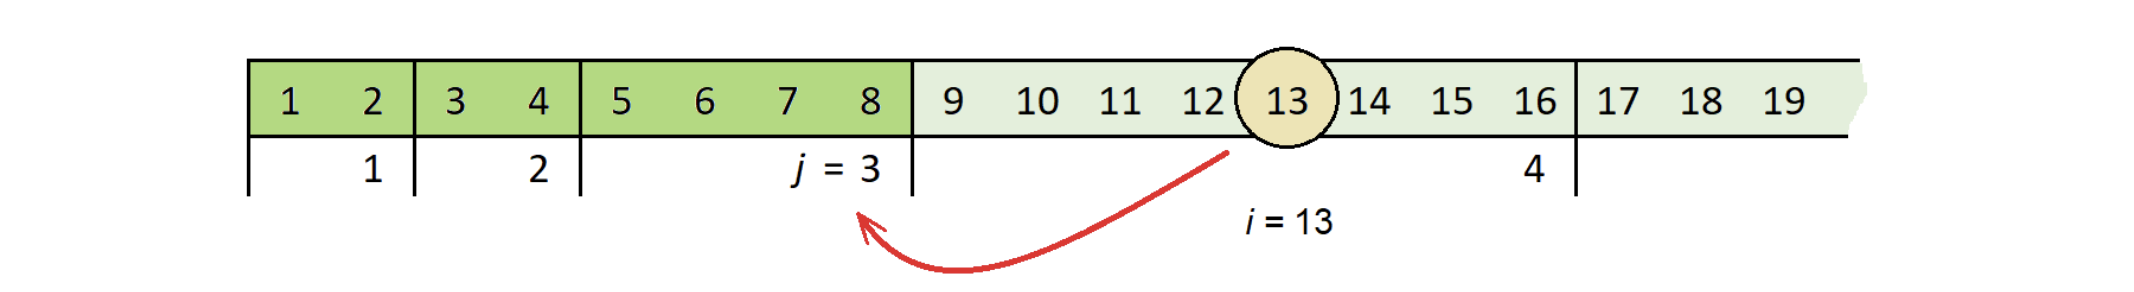
\includegraphics[width=15cm]{chapters/boosting/images/ordered_boost.png}

\subsection*{Модифицированный алгоритм градиентного бустинга в CatBoost}

\begin{tcolorbox}[colback=Lavender!10, colframe=Lavender]
\begin{enumerate}
\item Сгенерировать случайные перестановки \(\sigma_0, \sigma_1, \ldots, \sigma_s\);

\item \textbf{для всех} \(t = 1, \ldots, T\):
\begin{enumerate}
    \item выбрать перестановку \(\sigma_r\) случайно из \(\sigma_1, \ldots, \sigma_s\);
    \begin{flalign*}
    & g_{ti}^r := -\mathcal{L}'\left(a_{t-1}^{rj}(x_i), y_i\right) \quad \text{— несмещённый антиградиент;} &
    \end{flalign*}
    \begin{flalign*}
    & b_t := \arg\min_b \sum_{i=1}^{\ell} \left(b(x_i) - g_{ti}^r\right)^2; &
    \end{flalign*}
    \textbf{для всех} деревьев \(b_t^{rj}\), \(r = 1, \ldots, s\), \(2^j \leq \ell\):
    \begin{itemize}
        \item скопировать общую для них структуру дерева из \(b_t\);
        \item вычислить в листах \(b_t^{rj}\) средние по \(\{g_{ti}^r: x_i \in X^{rj}\}\);
    \end{itemize}
    \item вычислить в листах \(b_t\) средние по \(\{g_{ti}^0: x_i \in X^{0j}\}\);
    \item \textbf{GB part:} вычислить \(\alpha_t\) и обновить \(a_{t,i} := a_{t-1,i} + \alpha_t b_t(x_i)\);
\end{enumerate}
\end{enumerate}
\end{tcolorbox}

\subsection*{Обработка категориальных фичей}

Пусть $V$ — множество значений признака $f(x)$.\\

\textbf{Стандартные методы} либо громоздкие, либо переобучаются:
\begin{itemize}
    \item бинализация (one-hot encoding): \( b_v(x) = [f(x) = v] \);
    \item группирование (кластеризация) значений (LightGBM);
    \item статистика по целевому признаку - Target Statistics (TS):
    \begin{flalign*}
    & \tilde{f}(x_i) = \frac{\sum_{k=1}^{\ell}[f(x_k) = f(x_i)]y_k + \gamma p}{\sum_{k=1}^{\ell}[f(x_k) = f(x_i)] + \gamma} &
    \end{flalign*}
\end{itemize}

\textbf{CatBoost:}
\begin{itemize}
    \item статистика TS вычисляется по перестановкам \( X^{rj} \):
    $$
    \tilde{f}(x_i) = \frac{\sum_{x_k \in X^{rj}}[f(x_k) = f(x_i)]y_k + \gamma p}{\sum_{x_k \in X^{rj}}[f(x_k) = f(x_i)] + \gamma}, \quad j = \lfloor \log_2(i - 1) \rfloor
    $$
    \item конъюнкции категориальных признаков создаются «налёту» в процессе построения деревьев.
\end{itemize}

\subsection*{Особенности построения деревьев в CatBoost (Oblivious Decision Tree)}

Одной из ключевых особенностей алгоритма CatBoost является инновационный подход к построению деревьев решений. Деревья в CatBoost формируются по слоям, придерживаясь принципа: \textbf{\textit{все вершины одного уровня имеют одинаковый предикат}}. Это означает, что на каждом уровне дерева используется идентичный сплит для всех его вершин. Данный метод позволяет избавиться от сложных ветвлений в коде инференса модели и вместо этого использовать более эффективные битовые операции. Такое усовершенствование существенно ускоряет применение модели, особенно при работе с батчами данных.

Дерево глубины $H$, $D_v = \{0, 1\}$, для всех узлов уровня $h$ условие ветвления $f_h(x)$ одинаково; на уровне $h$ ровно $2^{h-1}$ вершин, $X$ делится на $2^H$ ячеек.

Классификатор задаётся \textit{таблицей решений} $B: \{0,1\}^H \to Y$:
$$
a(x) = B(f_1(x), \ldots, f_H(x)).
$$

\begin{figure}[ht]
    \centering
    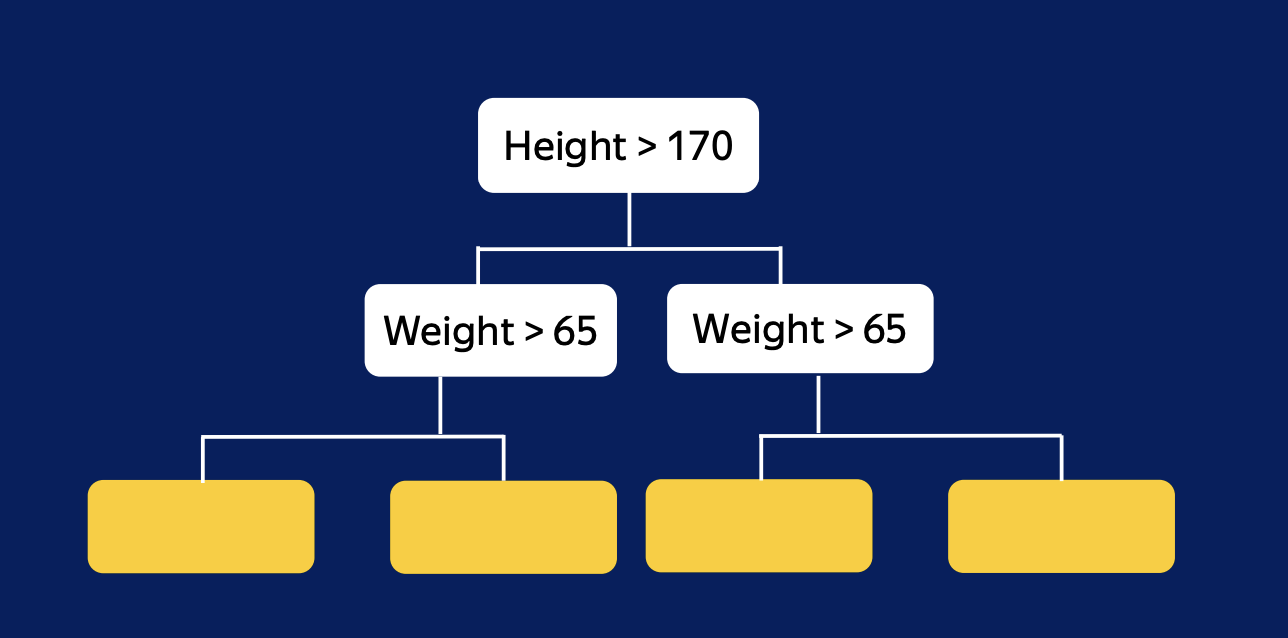
\includegraphics[width=15cm]{chapters/boosting/images/Tree.png}
    \caption{Пример сплита в слоях дерева в CatBoost}
\end{figure}

Кроме того, этот способ служит мощным средством регуляризации, обеспечивающим устойчивость модели к переобучению. Также данный подход позволяет всегда строить полные бинарные деревья (аналогично XGBoost, с тем различием, что CatBoost создаёт их даже в тех случаях, когда на некоторые поддеревья не попадает ни один объект из обучающей выборки). Основным критерием остановки процесса является ограничение на глубину деревьев.

\subsection*{Алгоритм обучения Oblivious Decision Tree}

\begin{tcolorbox}[colback=Lavender!10, colframe=Lavender]
\textbf{Вход:} выборка $X^\ell$; множество признаков $F$; глубина дерева $H$;\\
\textbf{Выход:} признаки $f_h, \ h = 1, \ldots, H$  таблица $B: \{0,1\}^H \to Y$;\\
\textbf{Для всех} $h = 1, \ldots, H$:\\
предикат с максимальным выигрышем определённости:
$$
f_h := \arg\max_{f \in \mathrm{bin}\{F\}} \text{Gain}(f_1, \ldots, f_{h-1}, f);
$$

\(\mathcal{B}(\beta) := \Phi(U_{H\beta}), \ \text{где} \ \Phi(U) = \text{avg}\{g_{ti}^r : x_i \in U\};\)
\end{tcolorbox}

$$
U_{h\beta} = \{x_i \in X^\ell : f_s(x_i) = \beta_s, \ s = 1 \ldots h\} \, \text{— выборка объектов } x_i,
\text{дошедших до вершины } \beta = (\beta_1, \ldots, \beta_h) \in \{0,1\}^h
$$

Выигрыш от ветвления на уровне \(h\) по всей выборке \(X^\ell\):
$$
\text{Gain}(f_1, \ldots, f_h) = \Phi(X^\ell) - \sum_{\beta \in \{0,1\}^h} \frac{|U_{h\beta}|}{\ell} \Phi(U_{h\beta})
$$

\subsection*{Основные преимущества CatBoost:}

\begin{itemize}
    \item \textbf{Эффективная работа с категориальными признаками.} CatBoost способен автоматически обрабатывать категориальные данные без необходимости их предварительного кодирования, такого как one-hot encoding.

    \item \textbf{Интегрированная обработка пропусков.} Алгоритм самостоятельно справляется с отсутствующими значениями.
    \item \textbf{Противодействие переобучению.} CatBoost применяет различные техники для предотвращения переобучения модели, включая мощные механизмы регуляризации и усреднение.

    \item \textbf{Высокая скорость и производительность.} В CatBoost реализованы множественные оптимизации, ускоряющие процесс обучения и предсказания. Он поддерживает многопоточную обработку и эффективно использует память.

    \item \textbf{Стабильность и воспроизводимость результатов.} Алгоритм гарантирует стабильные результаты даже при изменении порядка поступления входных данных, что важно для практического применения в реальных задачах.

\end{itemize}

\subsection*{Задача 1}

Предположим, что у вас есть обучающая выборка из 8 объектов. Покажите, как будут сформированы подвыборки $X^{rj} $ для объекта $x_5$ в одной из случайных перестановок, и какая модель будет использоваться для вычисления градиента на этом объекте.

\textbf{Решение:}

Используем одну случайную перестановку $\sigma$, которая для простоты совпадает с исходным порядком объектов: $\sigma = \left( x_1, \ x_2, \ x_3, \ x_4, \ x_5, \ x_6, \ x_7, \ x_8 \right)$.

\begin{enumerate}
\item  Определение значения $j$. Позиция объекта $x_5$ в перестановке: $i = 5$
   
   Вычисляем значение $j$:
   $$
   j = \left\lfloor \log_2(i - 1) \right\rfloor = \left\lfloor \log_2(5 - 1) \right\rfloor = \left\lfloor \log_2(4) \right\rfloor = 2
   $$
\item  Формирование подвыборки $X^{rj}$:

   Вычисляем размер подвыборки: $2^j = 2^2 = 4$

   Подвыборка $X^{rj}$ содержит первые $2^j = 4$ объекта из перестановки $\sigma$:
   $$
   X^{rj} = \left\{ x_1, \ x_2, \ x_3, \ x_4 \right\}
   $$

   Заметим, что объект $x_5$ не входит в эту подвыборку.
   
\item  Выбор модели для вычисления градиента на $x_5$:

   Модель $a_{t-1}^{rj}$ была обучена на подвыборке $X^{rj} = \left\{ x_1, \ x_2, \ x_3, \ x_4 \right\}$

   Поскольку $x_5 \notin X^{rj}$, модель $a_{t-1}^{rj}$ не была обучена на объекте $x_5$.

   Антиградиент на объекте $x_5$ вычисляется как:

   $$
   g_{t5}^r = -\mathcal{L}'\left( a_{t-1}^{rj}(x_5), \ y_5 \right)
   $$

   где \( a_{t-1}^{rj} \) — модель, обученная на подвыборке \( \left\{ x_1, \ x_2, \ x_3, \ x_4 \right\} \).

\end{enumerate}

\subsection*{Задача 2}

Опишите, как CatBoost вычисляет статистики по целевой переменной для категориальных признаков на примере:

\textbf{Дано}:
\begin{itemize}
    \item Перестановка объектов: $x_1, x_2, x_3, x_4, x_5, x_6$
    \item Значения признака  $f(x_i)$ и целевой переменной $y_i$
    \begin{table}[ht]
    \centering
    \begin{tabular}{c|c|c}
    Объект \( x_i \) & \( f(x_i) \) & \( y_i \) \\
    \hline
    \( x_1 \) & \( A \) & \( 1 \) \\
    \( x_2 \) & \( B \) & \( 0 \) \\
    \( x_3 \) & \( A \) & \( 1 \) \\
    \( x_4 \) & \( C \) & \( 0 \) \\
    \( x_5 \) & \( B \) & \( 1 \) \\
    \( x_6 \) & \( A \) & \( 0 \) \\
    \end{tabular}
    \end{table}
    \item Параметры: $\gamma = 1$, $p = 0{,}5$.
\end{itemize}

\textbf{Найти:} $\tilde{f}(x_5)$


\textbf{Решение:}

1. Определяем параметр $j$: 
$$
i = 5 \rightarrow j = \left\lfloor \log_2(i - 1) \right\rfloor = \left\lfloor \log_2(4) \right\rfloor = 2
$$

2. Формируем подвыборку $X^{rj}$:

   Количество объектов в подвыборке: $2^j = 2^2 = 4$. Значит, $X^{rj} = \{ x_1, \ x_2, \ x_3, \ x_4 \}$.

3. Выбираем объекты с \( f(x_k) = f(x_5) = B \):

   $\text{Совпадающие объекты} = x_2$, так как $f(x_2) = B$.

4. Получаем значения $y_k$ для совпадающих объектов: $y_2 = 0$.

5. Вычисляем сумму в числителе и знаменателе:
\begin{itemize}
   \item $\text{Числитель:} \sum\limits_{x_k \in X^{rj}} [f(x_k) = f(x_5)] y_k = y_2 = 0$
   \item $\text{Знаменатель:} \sum\limits_{x_k \in X^{rj}} [f(x_k) = f(x_5)] = 1$ 
\end{itemize}

6. Вычисляем $\tilde{f}(x_5)$:

$$
\tilde{f}(x_5) = \dfrac{\sum\limits_{x_k \in X^{rj}} [f(x_k) = f(x_5)] y_k + \gamma p}{\sum\limits_{x_k \in X^{rj}} [f(x_k) = f(x_5)] + \gamma} = \dfrac{0 + 1 \times 0{,}5}{1 + 1} = \dfrac{0{,}5}{2} = 0{,}25
$$

Ответ: $\tilde{f}(x_5) = 0{,}25$

\subsection*{Задача 3}

CatBoost использует особый тип деревьев решений, называемых небрежными деревьями (Oblivious Decision Trees), где на каждом уровне все узлы используют одинаковый предикат для разделения данных. Опишите основные преимущества использования обливиозных деревьев в CatBoost.

\textbf{Решение:}

\begin{enumerate}
    \item \textbf{Ускорение инференса:}
    \begin{itemize}
        \item Благодаря симметричной структуре дерева и одинаковым предикатам на каждом уровне, вычисления при предсказании можно оптимизировать.
        \item Использование битовых векторов и операций позволяет быстро определять путь по дереву и получать предсказание из таблицы решений.
    \end{itemize}
    \item \textbf{Оптимизация кода:}
    \begin{itemize}
        \item Упрощённая структура дерева снижает сложность кода и количество условных операторов.
        \item Это приводит к более эффективному использованию процессорного конвейера и кэшей.
    \end{itemize}
    \item \textbf{Регуляризация и устойчивость к переобучению:}
    \begin{itemize}
        \item Ограничение модели фиксированными предикатами на уровне уменьшает её сложность.
        \item Это служит формой регуляризации, помогая предотвратить переобучение на обучающей выборке.
    \end{itemize}
    \item \textbf{Предсказуемость и воспроизводимость:}
    \begin{itemize}
        \item Симметричная структура обеспечивает стабильность модели при различных изменениях в данных.
        \item Лёгкость воспроизведения результатов в различных средах и на различных устройствах.
    \end{itemize}
    \item \textbf{Совместимость с обработкой категориальных признаков:}
    \begin{itemize}
        \item Обливиозные деревья хорошо интегрируются с методами обработки категориальных признаков в CatBoost.
        \item Позволяют эффективно использовать конъюнкции (сочетания) признаков для повышения качества модели.
    \end{itemize}
\end{enumerate}

\section{LightGBM}

\subsection{Анализ сложности градиентного бустинга над решающими деревьями}

Самая вычислительно сложная часть градиентного бустинга над решающими деревьями (GBDT) является поиск наилучшей точки разбиения. В LightGBM используется \textbf{histogram-based} подход. Он заменяет истинные значения непрерывных признаков на группы ("бины") и для каждого признака строит гистограмму, где подсчитываются суммы весов для каждого бина. Вычислительная сложность в таком случае оказывается равной $\mathcal{O}(\#\text{bin}\cdot\#\text{features})$, что оказывается гораздо выгоднее алгоритма предварительной сортировки ($\mathcal{O}(\#\text{data}\cdot\#\text{features})$), поскольку обычно $\#\text{bin} \ll \#\text{data}$.

\subsection{Gradient-based One-Side Sampling (GOSS)}

Идея заключается в том, чтобы придумать способ, с помощью которого мы смогли бы находить наилучшее разбиение, не просматривая всю выборку. Аналогично алгоритму AdaBoost мы хотим присвоить каждому элементу выборки "вес", чтобы акцентировать внимание модели на них. В качестве этого веса может выступать градиент элемента. Так, например, данные с маленькими (по абсолютному значению) градиентами вносят малый вклад в ошибку, поэтому необязательно использовать их все.

GOSS предлагает следующий алгоритм сэмплирования: GOSS сначала сортирует данные в убывающем порядке по абсолютному значению градиентов и выбирает топ $a\times 100\%$ элементов. Далее он рандомно сэмплирует $b\times100\%$ элементов. Далее GOSS умножает часть с маленькими градиентами на константу $\frac{1 - a}{b}$ при вычислении прироста информации.

Более строго GBDT пытается выучить отображение из исходного пространства $\mathcal{X}^s$ в пространство градиентов $\mathcal{G}$. Предположим, мы имеем $n$ одинаковых независимо распределенных элементов $\{x_1, x_2, \ldots, x_n\}, \ x_i \in \mathcal{X}^s \ \forall i = \overline{1,n}$. Для каждой итерации градиентного бустинга определим $\{g_1, g_2, \ldots, g_n\}$ - антиградиенты loss-функции по отношению к текущему предсказанию модели. 

\par \textbf{Определение.} Пусть $\mathcal{X}$ - обучающая выборка в текущей ноде решающего дерева. Тогда прирост информации при разделении признака $j$ по значению $d$ для этой ноды определяется как

\begin{equation*}
    V_{j|\mathcal{X}}(d) = \frac{1}{|\mathcal{X}|}\left(\frac{\left(\sum\limits_{x_i\in \mathcal{X}: x_{ij} \leqslant d}g_i\right)^2}{n^j_l(d)} + \frac{\left(\sum\limits_{x_i\in \mathcal{X}: x_{ij} > d}g_i\right)^2}{n^j_r(d)}\right)
\end{equation*}

где $n^j_l(d) = |x_i\in \mathcal{X}: x_{ij} \leqslant d|, \ n^j_r(d) = |x_i\in \mathcal{X}: x_{ij} > d|$ Для каждого признака $j$ алгоритм выбирает $d_j^* = \arg\max\limits_dV_j(d)$ и вычисляет наибольший прирост информации $V_j(d_j^*)$. Далее данные делятся по признаку $j^*$ и по значению $d_j^*$ на правое и левое поддервья. В предложенном GOSS алгоритме выберем топ $a\times100\%$ элементов с наибольшим градиентом (по абсолютному значению) и обозначим это множество $A$. Далее из $\overline{A}$ случайно выберем $b\times|\overline{A}|$ элементов и обозначим $B$. Тогда оценка прироста информации имеет вид

\begin{equation*}
    \widetilde{V}_j(d) = \frac{1}{|\mathcal{X}|}\left(\frac{\left(\sum\limits_{x_i\in A_l}g_i + \frac{1 - a}{b}\sum\limits_{x_i\in B_l}g_i\right)^2}{n^j_l(d)} + \frac{\left(\sum\limits_{x_i\in A_r}g_i + \frac{1 - a}{b}\sum\limits_{x_i\in B_r}g_i\right)^2}{n^j_r(d)}\right),
\end{equation*}

где $A_l = \{x_i \in A: x_{ij} < d\}, \ A_r = \{x_i \in A: x_{ij} > d\}, B_l = \{x_i \in B: x_{ij} \leqslant d\}, \ B_r = \{x_i \in B: x_{ij} > d\}$.

То есть в GOSS мы используем оценку прироста информации $\widetilde{V}_j(d)$, рассчитанную по меньшему датасету, нежели точную $V_j(d)$. При этом согласно утверждению следующей теоремы, используя оценку $\widetilde{V}_j(d)$ вместо $V_j(d)$ мы не сильно проигрывает в точности:

\par \textbf{Теорема.} Обозначим ошибку аппроксимации GOSS как $\varepsilon (d) = |\widetilde{V}_j(d) - V_j(d)|$ и $\overline{g}_l^j(d) = \frac{\sum\limits_{x_i \in \mathcal{X}_l}|g_i|}{n^j_l(d)}, \ \overline{g}_r^j(d) = \frac{\sum\limits_{x_i \in \mathcal{X}_r}|g_i|}{n^j_r(d)}$. Тогда с вероятностью хотя бы $1 - \delta$ имеет место оценка

\begin{equation*}
    \varepsilon(d) \leqslant C_{a, b}^2 \ln \frac{1}{\delta} \cdot \max \left\{\frac{1}{n^j_l(d)}, \frac{1}{n^j_r(d)}\right\} + 2DC_{a, b}\sqrt{\frac{\ln \frac{1}{\delta}}{n}},
\end{equation*}

где $C_{a. b} = \frac{1 - a}{\sqrt{b}}\max_{x_i \in \overline{A}}|g_i|$ и $D = \max\left\{\overline{g}_l^j(d), \overline{g}_r^j(d)\right\}$. 

Из данной теоремы следует асимптотическая оценка GOSS $\mathcal{O}\left(\frac{1}{n^j_l(d)} + \frac{1}{n^j_r(d)} + \frac{1}{\sqrt{n}}\right)$. Поэтому если разбиения будут не слишком несбалансированными (то есть $n^j_l(d) \geqslant \mathcal{O}(\sqrt{n})$ и $n^j_r(d) \geqslant \mathcal{O}(\sqrt{n})$), то общая асимптотика будет составлять $\mathcal{O}\left(\frac{1}{\sqrt{n}}\right) \underset{n\rightarrow \infty}{\rightarrow} 0$. То есть при большом количестве данных приближение будет достаточно точным.

Обобщающая способность GOSS будет также близка к алгоритму с "честным" приростом информации. $\varepsilon_{\text{gen}}^{\text{GOSS}}(d) = |\widetilde{V}_j(d) - V_*(d)| \leqslant |\widetilde{V}_j(d) - V_j(d)| + |V_j(d) - V_*(d)| = \varepsilon_{\text{GOSS}}(d) + \varepsilon_{\text{gen}}(d)$.


\subsection{Exclusive Feature Bundling (EFB)}

Зачастую, датасеты большой размерности являются сильно разреженными, возникает мысль, что возможно уменьшить количество признаков, не сильно теряя при этом в точности. В частности, в разреженном пространстве зачастую встречаются взаимоисключающие признаки, то есть признаки, которые не могут быть ненулевыми одновременно. Такие признаки можно объединить в один (exclusive feature bundle). Соответственно, гистограмма из подпункта \textbf{1.1}, построенная на этих объединенных признаках имеет асимптотику $\mathcal{O}(\#\text{data}\times\#\text{bundle})$, вместо $\mathcal{O}(\#\text{data}\times\#\text{feature})$, что значительно быстрее при $\text{\#bundle} \ll \#\text{feature}$.

Сведем задачу разделения на такие $\text{bundle}$ к задаче раскраски графа (NP-Hard), признаки будем считать вершинами и ребро будем проводить между признаками, которые не являются взаимоисключающими. Точного полиномиального решения на текущий момент не существует, тем не менее задачу можно достаточно хорошо решить с помощью жадного алгоритма. Более того, обычно существует довольно много признаков, которые хотя и не являются на 100\% взаимоисключающими, но редко принимают ненулевые значения одновременно. Если наш алгоритм сможет разрешить небольшую долю конфликтов, мы сможем мы сможем получить еще меньшее количество bundles признаков и еще больше повысить эффективность вычислений. Такая процедура повлияет на точность при обучении не более чем $\mathcal{O}\left([(1-\gamma)n]^{\frac{2}{3}}\right)$, где $\gamma$ - максимальная частота конфликтов в каждом bundle.

Сформулируем итоговый алгоритм. Строим граф признаков с весами на ребрах, соответствующими общему числу конфликтов между признаками. Далее сортируем признаки по количеству соседей, с которыми есть конфликты в убывающем порядке, наконец, для каждого признака из упорядоченного списка проверяется, можно ли добавить признак в существующие bundles с минимальным конфликтом (контролируется параметром $\gamma$), иначе создается новый bundle. Общая сложность алгоритма - $\mathcal{O}(\#\text{feature}^2)$.

Далее нам надо понять, как правильно объединять признаки в один bundle, то есть по значению признака в bundle мы должны уметь определить исходное значение объединенных признаков. Это может быть сделано с помощью добавления смещения к признакам. Например, признак $A$ принимает значения из диапазона $[0, 10)$, а признак $B$ - из $[0, 20)$. Добавим смещение признаку $B$, теперь он принимает значения из диапазона $[10, 30)$. После объединения признаков $A$ и $B$ полученный признак будет принимать значения в диапазоне $[0, 30)$.

\subsection{Задачи}

\begin{enumerate}
    \item Обычно в методах градиентного бустинга стараются строить неглубокие деревья, чтобы не переобучиться на обучающей выборке и ускорить время обучения. Сохраняется ли это в LightGBM? Почему?

    Ответ: Нет, это нарушается в LightGBM реализации градиентного бустинга. Дело в другой стратегии роста - $\text{leaf-wise growth}$. Глядя на функционал прироста информации видно, что каждый раз выборка делится на одну часть с большими градиентами и вторую часть, с маленькими градиентами. Данные с маленькими градиентами уже вносят малый вклад в ошибку и дальше разбивать их не так информативно. LightGBM на каждом шаге выбирает наиболее оптимальное разбиение, не обращая внимание на сбалансированность получающегося дерева, из-за чего зачастую получаются глубокие и несбалансированные деревья.

    \item В GOSS при подсчете оценки прироста информации мы домножаем на множитель $\frac{1-a}{b}$. Зачем это нужно и что будет, если это домножение не производить?

    Ответ: Если мы просто уменьшим количество данных с малыми градиентами, это исказит относительную важность этих объектов в функции потерь. Масштабирование градиентов увеличивает вклад выбранных объектов с малыми градиентами так, чтобы их совокупный эффект оставался пропорциональным их изначальной доле в данных. Если множитель не использовать, объекты с большими градиентами будут еще сильнее доминировать при построении дерева. Модель будет чрезмерно подстраиваться под сложные примеры, пренебрегая общей точностью и, скорее всего, ухудшая обобщающую способность.

    \item В чем важность параметра $\text{min\_data\_in\_leaf}$ параметра в LightGBM, к чему могут привести его высокие и низкие значения? А параметра \newline $\text{num\_leaves}$?

    Ответ: \begin{enumerate}
        \item $\text{min\_data\_in\_leaf}$ - отвечает за минимальное количество элементов выборки в каждом листе. Чем выше этот параметр, тем более модель устойчива к зашумленным данным. Слишком большие значения, однако, могут приводить к снижению чувствительности модели сложных зависимостей, ухудшая качество предсказания. Слишком малые значения параметра, напротив, позволяют выучить достаточно сложные зависимости, однако возрастает вероятность переобучения.

        \item $\text{num\_leaves}$ - отвечает за максимальное количество листьев дерева. Аналогично предыдущему признаку регулирует сложность модели. Чем больше листьев - тем более сложные зависимости между признаками и целевой переменной может улавливать дерево, однако высока вероятность переобучиться. И напротив, чем меньше листьев, тем модель более устойчива к переобучению и к шума и тем хуже она справляется со сложными зависимостями.
    \end{enumerate}
\end{enumerate}